\documentclass[letterpaper,11pt]{article}
\usepackage[brazil]{babel}
\usepackage[T1]{fontenc}
\usepackage{ae}
\usepackage[utf8]{inputenc}
\usepackage[dvipsnames]{color}
\usepackage{graphicx}
\usepackage{epsfig}
\usepackage{amssymb, amsmath, amsfonts}
\usepackage{graphicx}
\bibliographystyle{plain}
\topmargin 0 cm
\hoffset -1 cm
\voffset 0 cm
\evensidemargin 0 cm
\oddsidemargin 0 cm
\setlength{\textwidth}{18 cm}
\setlength{\textheight}{21 cm}

\title{ As cr\^{o}nicas de Medrash }
\author{ Grupo 1 }
\date{}

\begin{document}
\begin{center}
\begin{minipage}{2.4 cm}
\begin{center}

\includegraphics{logo.png}
\end{center}
\end{minipage}
\begin{minipage}{12 cm}
\begin{center}
\Large
UNIVERSIDADE ESTADUAL DE CAMPINAS \\
FACULDADE DE ENGENHARIA ELÉTRICA E DE COMPUTAÇÃO
\end{center}
\end{minipage}
\end{center}

\vspace{6 cm}
\begin{center}
{\bf \large GAME DESIGN DOCUMENT}
\vspace{0.5 cm}

Introdução ao Projeto de Jogos Digitais (IA369A) \\
Professor: José Mario De Martino \\
Primeiro Semestre de 2012
\end{center}
\vspace{3 cm}
\begin{flushright}
{\bf Grupo 1A} \\
Edgar Armeliato \\
Fernanda Leal \\
Harlei Miguel de Arruda Leite \\
Julián Prada Sanmiguel \\
Lauro Américo dos Santos \\
Maria Fernanda Rodriguez \\
Paúl Mejia \\
Rodrigo Mologni \\
Rodrigo Aparecido Morbach \\
Tiago Cinto \\
Thiago Cavalcante
\end{flushright}

\newpage
\tableofcontents
\newpage

{\bf Proposta do Jogo - Grupo 1}

\section{Nome do Jogo}

As Crônicas de Medrash

\section{Visão Global do Jogo}

\subsection{Enredo}
Medrash, um jovem caçador da pequena e pacífica tribo Ari, ao retornar de uma caçada na noite anterior, encontra sua tribo completamente devastada na manhã seguinte. Nela, há apenas um sobrevivente dentre os feridos agonizantes, seu amigo Gardain, um dos mais fortes guerreiros locais, que mesmo gravemente machucado, consegue contar à Medrash que na noite anterior eles foram surpreendidos por guerreiros da poderosa tribo Luskan – a mais temida dentre todas da região – e que não tiveram chance de se defender do ataque. Os sobreviventes de sua tribo foram levados pelos luskans para serem escravizados. Este ataque havia sido orquestrado por seu arqui-inimigo, Balasar, líder da tribo inimiga. Como se não bastasse a tragédia ocorrida, Medrash ainda é informado que os luskans haviam levado dentre os prisioneiros sua amada esposa, Sora.  Desesperado, Medrash inicia uma jornada contra o tempo em direção aos inimigos, rastreando a trilha deixada por eles. \\
Ao final da trilha, após lutar contra as mais diversas adversidades e perigos, Medrash finalmente alcança seus inimigos; entretanto, antes que pudesse tomar qualquer atitude, ele  surpreende-se com o que presencia diante de seus próprios olhos: os aliados, da tribo Mara-kai, estão sob pesado ataque dos luskans, estratégia semelhante ao que havia ocorrido com sua tribo natal anteriormente. Após o cessar fogo e retirada inimiga, a devastação e o caos são eminentes entre as dependências dos mara-kais. Em sua busca por sobreviventes, Medrash encontra Rangrim, líder da tribo aliada ferido, que lhe dá a terrível notícia de que os inimigos marcham agora rumo à Akanul – a última e mais importante das tribos aliadas locais. Como já não haviam mais guerreiros das tribos atacadas que poderiam ajudar Medrash em um contra-ataque para libertar os membros capturados, a única alternativa agora seria chegar à Akanul antes dela ser destruída pelos luskans. Para isto, Rangrim indica um atalho pelas montanhas frias e selvagens Kabalus. \\
Felizmente, após a difícil e perigosa jornada pelas montanhas, Medrash chega a tempo de informar à tribo da invasão que eles sofrerão. Preparados, os akanuls conseguem se defender e evitam que seus membros sejam levados para a escravidão. Em busca de resgatar seus amigos e sua querida amada, Medrash e os demais guerreiros partem em direção à Luskan. Após vários confrontos com os guerreiros luskans, Medrash e os demais aliados conseguem libertar os escravos; contudo, sua amada não encontrava-se junto a eles: Sora estava com o temido Balasar. Para resgatá-la, Medrash terá que enfrentar seu algoz sozinho em uma batalha corpo-a-corpo de vida ou morte.

\section{Personagens}

\section{Fases}
\subsection{Fase 1}
O cenário geral representa uma floresta de coníferas. Esta será dividida em quatro 
regiões: A, B, C e D, tal como ilustrado na Figura 2. A região A localiza-se na parte 
mais alta da floresta, onde encontra-se a tribo do personagem principal e é a posição 
que este inicia no jogo. Para deslocar-se entre as regiões A e B, o personagem deverá 
descer a montanha saltando entre as pedras. O personagem deverá morrer em caso de 
quedas altas. Como dificuldade de percurso, haverá pedras soltas que exigirão rapidez 
do jogador. Esta região de transição também estará infestada de cobras. A região B 
será plana e composta por muitas árvores. Esta área será dominada por ursos e em 
algumas árvores haverá cachos de abelhas. Na região C há um rio repleto de jacarés. 
O personagem poderá atravessá-lo andando (não correndo), já que as águas são baixas, 
ou pulando sobre as pedras no rio. Por fim, na região D, é onde encontra-se o último 
inimigo do personagem, o tigre.

\begin{figure}[!ht]
 \centering
 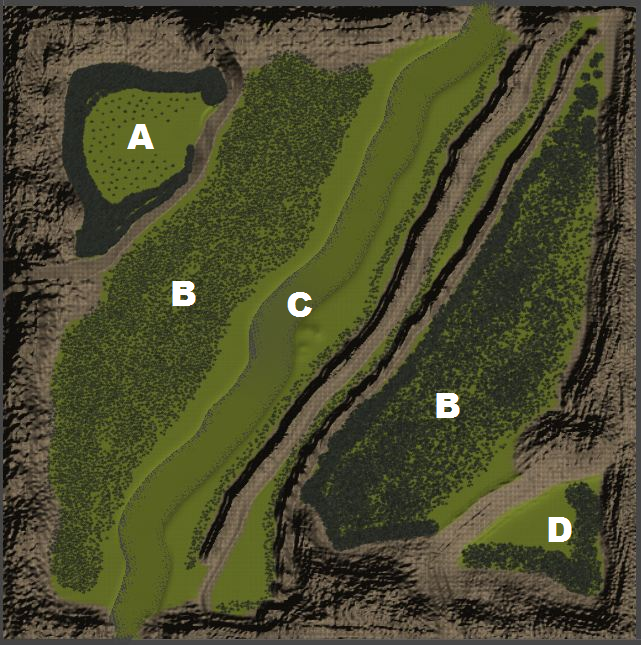
\includegraphics[scale=1]{cenario01.png}
 \caption{Esboço do cenário geral da primeira fase.}
 \label{img:cenario01}
\end{figure}
\section{Fluxo do Jogo}

\section{Mecânica do Jogo}


Nesta sessão descreveremos as regras de interação entre o jogador e o jogo.

\subsection {Mecânica Basica}

O jogador irá passar por mapas do jogo tendo a liberdade de andar em qualquer direção até que encontre um checkpoint que estará em uma região do mapa que não permite a volta do personagem a área anterior.

\subsubsection {Controles}

O jogador pode movimentar o personagem pelo cenário através das setas direcionais. Para as demais interações serão utilizadas as teclas ''A'', ''S'' e ''D''.
\begin{itemize}
\item ''D'' é o botão de ação, quando existem inimigos perto ele ataca, caso contrario ele realiza a interação com o cenário e outros personagens.
\item ''S'' é o botão de pulo, faz com que o personagem pule.
\item ''A'' é o botão de defesa, quando não for possível sair da frente de um ataque a tecla ''A'' pode ser usada para se defender.
\end{itemize}

\subsubsection {Deslocamento}

O personagem principal se desloca inicialmente correndo. Conforme este perde energia passa a correr mais devagar até que atinja um nível crítico
onde o personagem passa a andar apenas

\subsubsection {Inimigos e Desafios}

Nos mapas vão existir diversos inimigos que podem detectar o jogador se este chegar muito próximo 
e então dão inicio a uma perseguição, assim que o jogador se afasta a uma determinada distância esses voltam ao seu estado inicial. 

Estes inimigos quando próximos do jogador irão ataca-lo possibilitando que o jogador também faça o mesmo. 
Adicionalmente no final de cada mapa haverá um desafio extra como um inimigo mais forte ou uma batalha.  

\subsubsection {Interação com o Cenário}

Além dos inimigos o personagem principal poderá interagir com partes do cenário e outros personagens para completar os
desafios propostos.

\subsection {Combate}
\subsubsection{Inimigos}
Ao se aproximar dos inimigos, estes irão atacar o personagem principal. O personagem principal pode então pressionar a tecla ''D'' para atacar o inimigo mais 
próximo.

Os ataques dos inimigos serão periódicos podendo ser defendidos utilizando a tecla ''A'', que irá reduzir o dano causado, ou podem ser esquivados utilizando as 
setas direcionais para sair da região de efeito do ataque.

\subsubsection {Armas}
O personagem principal começa armado com um porrete de madeira. Durante a primeira fase este pode pegar uma lança que irá facilitar no combate com o tigre. 

Na segunda fase haverá um bastão em chamas que, entre outros usos, espanta os animais que estão próximos.

\subsection {Dificuldade}

O jogo tem apenas um modo de dificuldade. Os desafios propostos aumentam de dificuldade conforme a progressão dentro de cada fase.

De uma fase para outra são introduzidas novas mecânicas de jogo aumentando o grau de dificuldade e criando um incentivo para que o jogador 
não perca o interesse pelo jogo.

\subsection {Vide e Energia}

Existem duas barras principais durante o jogo, as barras de vida e energia. 

A barra de vida indica a saúde do personagem, esta barra diminui quando
o personagem sofre ataques dos inimigos e aumenta quando esse derrota os inimigos.

A barra de energia representa um desafio extra que depende da fase, esta barra diminui conforme o deslocamento do personagem e aumenta quando o 
mesmo cumpre alguns objetivos na fase.

\subsection {Salvar e Carregar o jogo}
?
\section{Interface}

Nesta seção, descrevemos os elementos de interação entre o jogador e o
jogo.

\subsection{HUD}

A tela do jogador terá as informações a seguir, seguindo o modelo da
Figura \ref{fig:hud}
\begin{figure}[!ht]
 \centering
 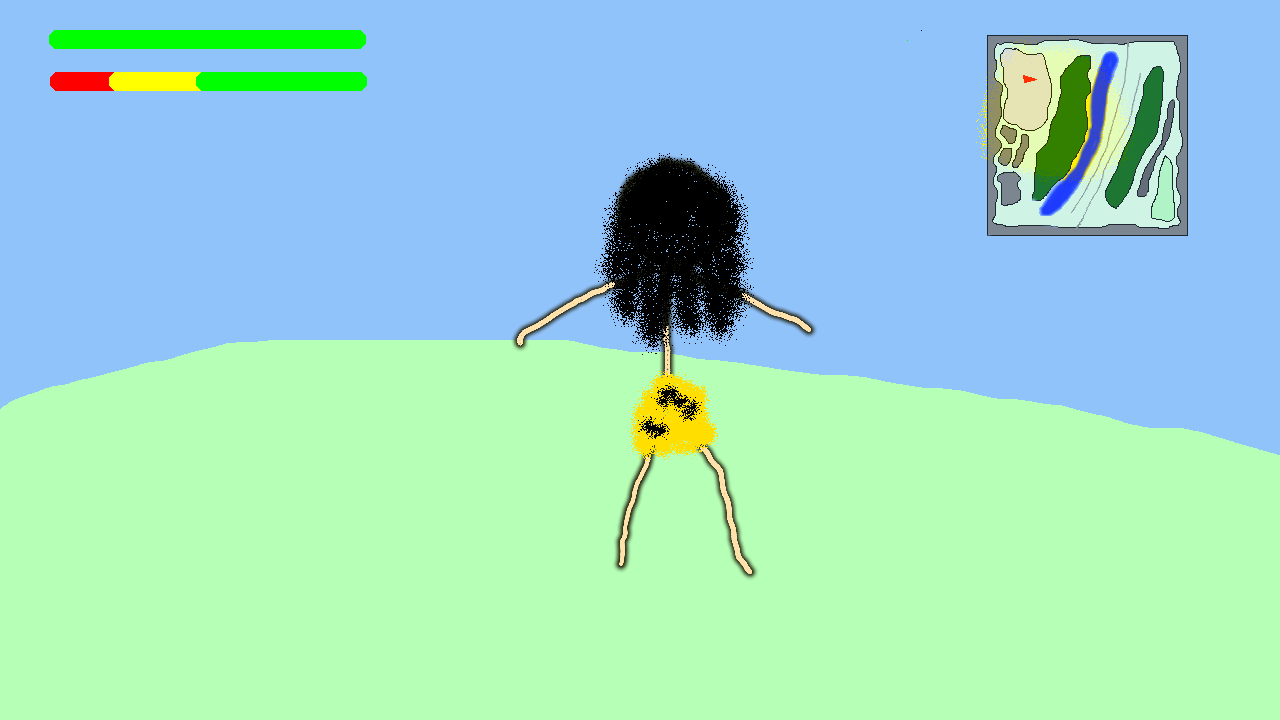
\includegraphics[scale=0.39]{hud.png}
 \caption{HUD}
 \label{fig:hud}
\end{figure}
\begin{enumerate}
 \item {\bf Barra de Vida:} Canto superior esquerdo da tela, no 
formato de uma barra horizontal. 
 \item {\bf Barra de Energia/Temperatura:} Quando houver esta barra,
ela estará no canto superior esquerdo da tela,
abaixo da barra de vida.
 \item {\bf Minimapa:} Canto superior direito, em forma de quadrado.
Será fixo e semi-transparente. Mostrará um esboço do mapa e um triângulo
indicando a posição e direção de Medrash. Existirá apenas na primeira fase.
\end{enumerate}

\subsection{Menus}

O jogo terá apenas dois menus. Um deles será o menu principal do jogo, e o 
outro será o menu de pausa.

\subsubsection{Menu Principal}

O menu principal terá as seguintes opções:
\begin{itemize}
 \item {\bf Começar novo jogo:} Apaga todas informações sobre o jogo atual,
se houver, e inicia um novo jogo.
 \item {\bf Continuar jogo:} Se houver um jogo em progresso, permite que
o usuário continue o mesmo. Caso contrário, esta opção estará desativada.
 \item {\bf Sair do jogo:} Sai do jogo, finalizando o software.
\end{itemize}

\subsubsection{Menu de Pausa}
O menu de pausa só pode ser acessado durante o jogo, e contém as seguintes
opções:
\begin{itemize}
 \item {\bf Continuar o jogo:} Sai do menu de pausa.
 \item {\bf Voltar ao menu principal:} Sai do jogo e volta ao menu 
principal. Não salva o jogo.
 \item {\bf Sair do jogo:} Sai do jogo e finaliza o software.
\end{itemize}


\section{Músicas e Efeitos Sonoros}

\section{Inteligência Artificial}

\subsection{Cobra}

A cobra rasteja aleatoriamente no cenário. A partir do momento que
Medrash entra no campo de deteção da cobra, esta fica em posição
de ataque. Se Medrash se aproximar ainda mais, ela o atacará.
A única forma de Medrash evitar este ataque será esquivando. O ataque
ignora a defesa de Medrash.
Uma vez que Medrash saia se afaste do campo de deteção da cobra, ela
voltará a patrulhar.

\begin{center}
 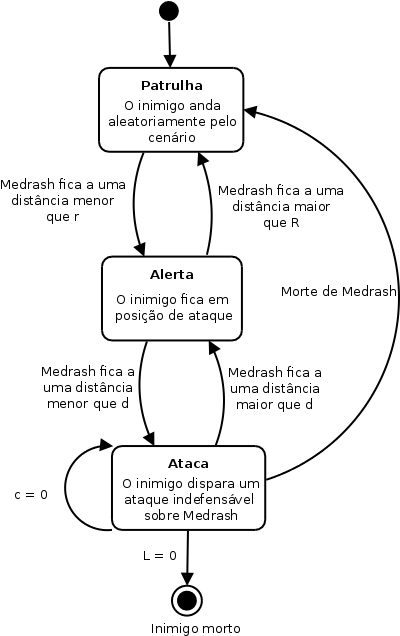
\includegraphics[scale=0.6]{ia_cobra.png}
\end{center}

\subsection{Enxame de abelhas}

O enxame de abelhas fica aglomerado na colméia. Quando Medrash se
aproxima o suficiente da colméia, o enxame começa a perseguí-lo.
A única opção de Medrash é fugir, pois as abelhas não podem ser atacadas.
Quando Medrash se afastar o suficiente da colméia, o enxame deixa
de perseguí-lo.
Se o enxame se aproximar de Medrash, irá atacá-lo.

\begin{center}
 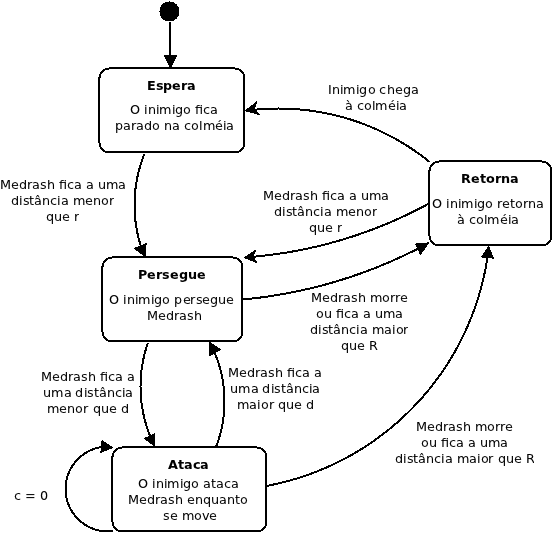
\includegraphics[scale=0.7]{ia_enxame.png}
\end{center}

\subsection{Jacaré}

O jacaré fica nas proximidades do rio. Se Medrash se aproximar dele,
este o perseguirá. Se Medrash se afastar o suficiente dele, o jacaré voltará às proximidades de seu ponto inicial.
O jacaré se movimenta dentro e fora do rio. Caso ele fique próximo de
Medrash, irá atacá-lo. Se sua barra de vida estiver baixa, ele atacará
múltiplas vezes.

\begin{center}
 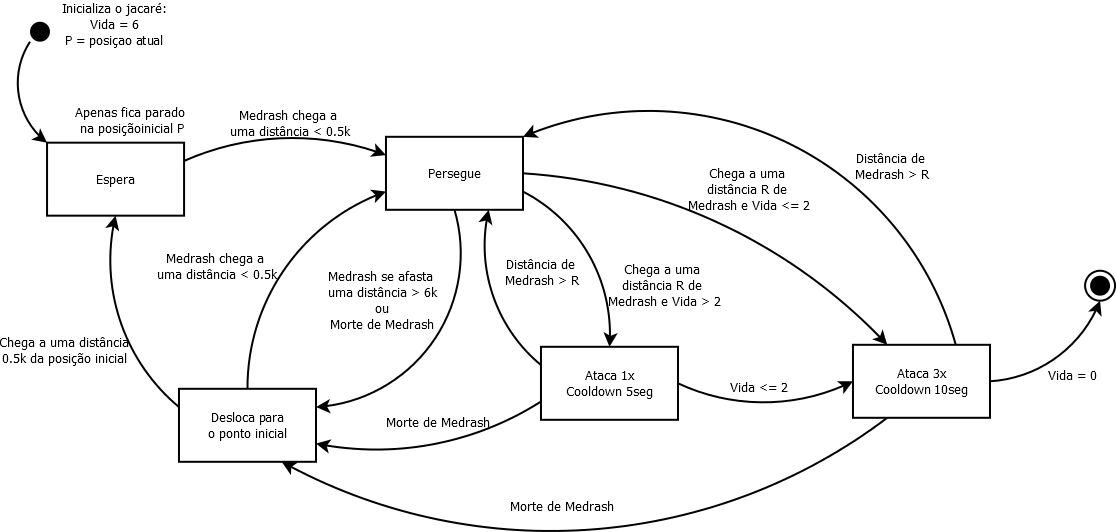
\includegraphics[scale=0.6]{ia_jacare.png}
\end{center}

\subsection{Tigre (1$^\circ$ chefe)}

Sendo o chefe da primeira fase, o tigre segue uma estratégia mais agressiva.
Inicialmente, ele corre em volta de Medrash, mantendo-se à uma distância
 segura. Após algum tempo, ele correrá em direção ao Medrash. Caso se
 aproxime, ele o atacará. Se Medrash conseguir se afastar por tempo
 suficiente, o tigre voltará a circular Medrash.
Periodicamente o tigre andará devagar para recuperar sua energia. Nesse
período, o Medrash consegue alcança-lo, e atacá-lo. Ao ser atacado, o tigre
volta a circular.
Quando sua barra de vida estiver baixa, o tigre também irá preparar um
bote. Ele ficará esperando Medrash se aproximar. Caso Medrash se aproxime,
 ele atacará com um salto. Se Medrash permanecer afastado por tempo 
suficiente, ele voltará a circular.

\begin{center}
 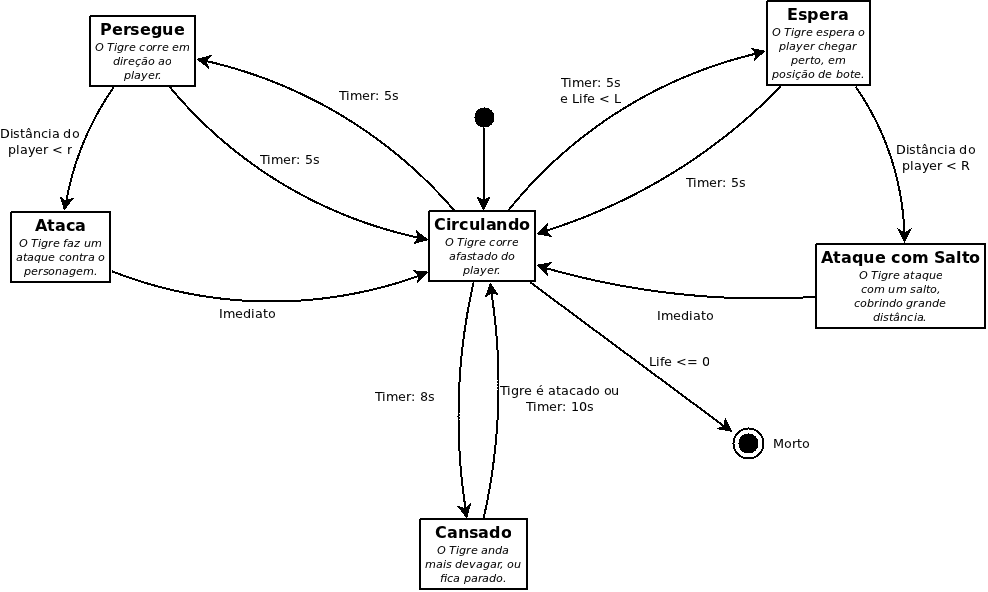
\includegraphics[scale=0.44]{ia_tigre.png}
\end{center}

\subsection{Urso}

O urso fica patrulando na floresta. Caso Medrash entre no raio de deteção
do urso, este o perseguirá. Para fugir do urso, Medrash deve ficar a uma
distância bem maior que o raio de deteção.
Se o urso se aproximar muito de Medrash, este será atacado. Enquanto estiver
próximo, o urso, periodicamente, irá se defender.

\begin{center}
 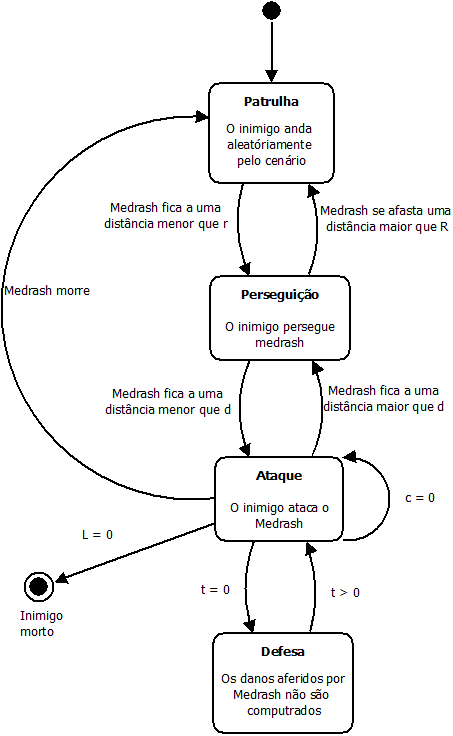
\includegraphics[scale=0.5]{ia_urso.png}
\end{center}

\section{Detalhamento Técnico}

\section{Testes}


\end{document}

